
\documentclass[doc,helv,longtable]{article}
\usepackage[spanish]{babel}

\usepackage[hidelinks]{hyperref}


% \usepackage{palatino} % Esta es genial!
% \linespread{1.05} % Palatino queda mejor con un poco más de interlineado.
%\usepackage{times} % Times New Roman.

\usepackage{graphicx}
\usepackage{verbatim}
\usepackage{setspace}
\usepackage{url}
\usepackage[utf8]{inputenc}

% Sarpadísima tipografía para listings y \texttt
\usepackage{inconsolata}

\usepackage{xcolor}

% Para ejemplos de código.
\usepackage{listings}
\lstset{ 
    % language=Prolog,    
    basicstyle=\ttfamily\small, % Usa inconsolata
    identifierstyle=\ttfamily,
    keywordstyle=\color[rgb]{0,0,1},
    commentstyle=\color[rgb]{0.133,0.545,0.133},
    stringstyle=\color[rgb]{0.627,0.126,0.941},
    morekeywords={true,false},
    showstringspaces=false,     % No muestra underscores en los espacios de los strings.
    backgroundcolor=\color{gray!10}, % Un color suave de fondo (menos chocante que el frame=single)
    breaklines=true,            % Wrappea las lineas automáticamente.
    numbers=left,                    % where to put the line-numbers; possible values are (none, left, right)
    numbersep=5pt,                   % how far the line-numbers are from the code
    numberstyle=\tiny\color{gray},
    belowskip=0pt               % Reduce el espacio entre un listing y el párrafo siguiente
    %frame=single               % Un recuadro en los listings.
}

% Para tener cabecera y pie de página con un estilo personalizado.
\usepackage{fancyhdr}

\bibliographystyle{IEEEtran}

\begin{document}

% Encabezado: sección a la derecha.
% Pie de página: número de página a la derecha.

\pagestyle{fancy}
\renewcommand{\sectionmark}[1]{\markboth{}{\thesection\ \ #1}}
\lhead{}
\chead{}
\rhead{\rightmark}
\lfoot{}
\cfoot{}
\rfoot{\thepage}

% ---------------------- ~Encabezado y pie de página ----------------------

\title{Informe TP Profesional - Invisible.js}
% \maketitle

% ------------------------------- Carátula --------------------------------

\begin{titlepage}

\thispagestyle{empty}

% Logo facultad.
\begin{center}

\includegraphics[scale=0.55]{./fiuba}\\
\textsc{\Large Universidad de Buenos Aires}\\[0.2cm]
\textsc{\Large Facultad de Ingeniería}\\[1.5cm]

% Título central.

\textsc{\large Trabajo Profesional de Ingeniería en Informática} \\[0.3cm]
% \textsc{\large Trabajo Práctico} \\[0.5cm]

\rule{\linewidth}{0.5mm} \\[0.4cm]
{\huge \bfseries Invisible.js} \\[0.3cm]
% {\Large \bfseries Introducción al lenguaje y a la programación lógica}
\rule{\linewidth}{0.5mm} \\ [2cm]

% \vfill

% Tabla de integrantes.
\begin{flushleft}
\Large\center\emph{Integrantes} \\[0.2cm]

% Separación entre columnas.
\begin{tabular}{lll}
Martín Paulucci & 88509 & martin.c.paulucci@gmail.com \\
Facundo Olano & 87712 & facundo.olano@gmail.com \\
\end{tabular}
\end{flushleft}

\end{center}
\end{titlepage}

% ------------------------------- ~Carátula -------------------------------

% -------------------------------- Índice ---------------------------------

% Hago que las páginas se comiencen a contar a partir de aquí.
\setcounter{page}{1}

% Índice.
\tableofcontents
\newpage

% -------------------------------- ~Índice --------------------------------

% ----------------------------- Inicio del tp -----------------------------

\clearpage  

% Saca la indentación de los párrafos y añade un espacio entre cada uno.
\setlength{\parindent}{0pt}
\setlength{\parskip}{2ex plus 0.5ex minus 0.2ex}

% Luego del índice, links con color.
\hypersetup{
linkcolor=red
}

\section{Introducción}

A medida que avanzan las aplicaciones web, se pasó progresivamente de arquitecturas en las que todo el procesamiento se hacía del lado del servidor, hacia otras en las que el cliente es cada vez más complejo, al punto de que mucho del trabajo hoy en día lo realiza el browser más que el servidor\cite{jsmvcvs}. Una vez superado el uso de CGI scripts y aplicaciones desestructuradas en lenguajes como PHP y ASP, se estandarizó el uso de frameworks MVC en el servidor, como Rails o Django. Estos se suelen complementar con bibliotecas como JQuery para mejorar la interfaz de usuario y la presentación. 

En la medida en que se requerían interfaces “ricas”\cite{rich}, actualizaciones en tiempo real, etc., aumentaron el tamaño y la complejidad del código del cliente. Se introdujeron entonces herramientas para resolver esta parte del problema\cite{richjs}: frameworks MVC, como backbone.js\cite{backbone}, para estructurar modelos en el cliente; MVVM, que facilita construir vistas responsivas a eventos, como lo hace knockout.js\cite{knockout}, etc. Todas estas arquitecturas se suelen agrupar como MV*\cite{mvw}.

Es fácil ver el problema de mantener dos estructuras de este estilo en paralelo en el cliente y el servidor. Por ejemplo, el programador tiene que cambiar de lenguaje al pasar de uno a otro, casi forzosamente hay duplicación de comportamiento entre los modelos en cada lado, un trabajo engorroso para manipular el DOM de las páginas para reflejar el estado en el servidor, no siempre se pueden reutilizar las plantillas (templates) con las que se arman las páginas, etc.\cite{wdsucks}

De aquí que resulte de interés encontrar la manera, no solo de sincronizar el estado, sino de reutilizar las definiciones de modelo, validaciones, etc., que hoy en día es casi forzoso duplicar. El objetivo de este Trabajo Profesional es construir una plataforma sobre la que el programador pueda solucionar esos problemas, reduciendo al mínimo la distinción que debe hacer entre el código de cliente y el de servidor. Una serie de recientes desarrollos hacen viable acercar esta meta, cuando no alcanzarla por completo. Es deseable:


\begin{itemize}
\item  Definir una sola vez modelos, validaciones, métodos y consultas a la base de datos, y poder usarlos indistintamente en cliente y servidor. Usando node.js\cite{node} se puede programar en JavaScript como lenguaje en el servidor, permitiendo reusar el código; a su vez, con CoffeeScript\cite{coffee} se puede alcanzar un nivel de expresividad similar al de lenguajes “tradicionales” de backend como Ruby o Python.
\item  Automatizar la actualización de la vista de acuerdo al estado de los datos, sean estos modificados en la vista por cualquier usuario o en el backend. Es decir, se ha de lograr una bidireccionalidad en la comunicación entre cliente y servidor (que el servidor pueda enviar información que no responda a ningún request); este problema se puede resolver con websockets\cite{websockets}.
\item  Definir los templates de las páginas una sola vez, pudiendo precargarlas en el servidor al entrar en una url específica, o actualizarlas arbitrariamente desde el cliente.

\end{itemize}


Para encarar con seriedad una nueva plataforma es fundamental tener un conocimiento cabal de la tecnología y alternativas disponibles actualmente. Para el caso de este trabajo es aún más importante siendo que ya existen frameworks con un enfoque similar al nuestro, y asimismo con distinta finalidad pero que resuelven parte de los mismos problemas, que se podrán reutilizar, o de los cuales extraer ideas y conclusiones. 

La primera parte del trabajo, entonces, consistirá en obtener ese conocimiento. En primera instancia, mediante la lectura de bibliografía pertinente, de investigación en blogs y sitios de tecnología, y de consultas a otros programadores, se seleccionará una lista de tecnologías y bibliotecas que nos parecen útiles para el trabajo posterior. Una vez definida esa lista, se pasará a realizar una serie de pruebas y prototipos sobre esas tecnologías, para extraer conclusiones útiles a nuestro proyecto.

De acuerdo a los resultados de este proceso, el resto del trabajo consistirá en:
\begin{itemize}
\item  Combinar, extender y/o completar los frameworks y tecnologías disponibles, implementando lo que sea necesario para alcanzar el mínimo grado de completitud esperado en un framework web.  
\item  Desarrollar una aplicación de prueba en el framework resultante.

\end{itemize}
\section{Investigación}
\subsection{CoffeeScript}


Por la naturaleza del trabajo propuesto, necesariamente se va a utilizar como lenguaje JavaScript en una medida importante; esto se debe a que es el único lenguaje que por ahora interpretan los navegadores web. Esto plantea un problema, ya que JavaScript excedió por completo su motivación original y adolece de varios problemas de diseño\cite{goodparts}. Esta situación se puede atenuar restringiendose a un subconjunto del lenguaje, que evite en la medida de lo posible sus aspectos problemáticos.

CoffeeScript es un lenguaje que compila a JavaScript (siguiendo fuertes convenciones de buenas prácticas para este lenguaje) y que pretende ocultar muchos de los inconvenientes de diseño mencionados, a la vez que presenta una sintaxis más expresiva (cercana a Python o Ruby). Todo esto lo convierte en una opción interesante, pero hay que sopesar las desventajas que acarrea: 
\begin{itemize}
\item  Como los browsers no interpretan CoffeeScript, el código escrito en este lenguaje que sea usado en el cliente tiene que ser previamente compilado a JavaScript. De esta forma  se agrega un paso adicional al ciclo de desarrollo. Sin embargo, hoy en día existen varias herramientas que facilitan los procesos de desarrollo, como Grunt\cite{grunt}.
\item  El código que se ejecuta finalmente es JavaScript, por lo tanto a la hora de debuggear, no va a estar disponible el código original sino el compilado. Este problema se puede solucionar con la utilización de Source Maps\cite{sourcemaps}.
\item  Podría resultar una mala decisión de diseño para una plataforma el imponer el uso de un lenguaje no convencional. 

\end{itemize}

\subsection{Comunicación Servidor-cliente}
El protocolo HTTP tiene una arquitectura Cliente-Servidor. Esto es, el método de funcionamiento es que el Cliente hace un pedido (request), el Servidor lo recibe y procesa, y envía una respuesta (response) al Cliente. Sin embargo, en tanto las aplicaciones web se complejizaron y sobre todo, con la difusión de los requests asincrónicos como medio para dinamizarlas, pasó a ser una necesidad el que el servidor envíe información hacia el cliente, sin que ésta sea una respuesta a un pedido. Esto permite implementar desde pequeñas notificaciones hasta complejas aplicaciones de tiempo real. Como se trata de un uso para el que el protocolo no estaba preparado, no hay aún una forma estándar de implementarlo, si bien existen soluciones parciales o aún en desarrollo para hacerlo\cite{wsvssse}.

Como el presente trabajo se propone desarrollar una plataforma en la que el programador pueda desentenderse de la diferencia entre cliente y servidor, se hace necesario que implemente la comunicación Servidor-Cliente en forma transparente al código de aplicación. Nótese que no es el objetivo del proyecto encontrar una solución general o ideal para este problema, si no aplicar las ya disponibles de la manera más simple para obtener el efecto deseado.

\subsubsection{Long-polling}
Long-Polling o Server Push\cite{longpolling} son nombres que se le dan comúnmente a la técnica de simular el envío de información desde el servidor al cliente que consiste en que el Cliente envíe un request asincrónico al Servidor, y que éste retenga la respuesta abierta hasta que tenga información que enviar. Se trata de un método ineficiente e inelegante, si bien la única opción disponible hasta hace poco.

\subsubsection{WebSockets}
La especificación de WebSockets presenta una API para establecer conexiones bidireccionales entre servidor y cliente, mucho más eficientes que las de HTTP\cite{websockets}. Es una tecnología de desarrollo reciente, y aún no está soportada por todos los browsers, y, al utilizar un protocolo distinto a HTTP, requiere mayor configuración y software específico en el servidor.

\subsubsection{Server-Sent Events}
Los Server-Sent Events\cite{sse} son otra tecnología que soporta el envío de información desde el Servidor al Cliente. Funcionan sobre HTTP, por lo que no tienen requerimientos especiales sobre los servidores, y su utilización resulta más simple que la de WebSockets\cite{congress}\cite{wsvssse2}. A diferencia de estos, no proveen comunicación bidireccional, es decir, es un canal para que el servidor envíe datos al cliente y no viceversa. Esto no es un gran problema, puesto que se pueden usar request tradicionales para la otra dirección, si bien con un costo mayor de recursos\cite{ssedownside}.

\subsubsection{socket.io}
socket.io\cite{socketio} es una biblioteca escrita en JavaScript, que provee una interfaz para comunicación bidireccional entre cliente y servidor, similar a la de WebSockets, y que puede variar la tecnología que usa para implementarla de acuerdo a las capacidades del navegador (por ejemplo, usar Long-Polling si éste no soporta WebSockets). Se trata de una opción ideal para resolver el problema en cuestión, con la salvedad de que es una biblioteca que requiere el uso de node.js, lo cual complejiza la configuración en los casos en que la aplicación utilice otra tecnología en el Servidor. Esto probablemente no sea un impedimento para este trabajo, puesto que implementar el Servidor con node.js es la única manera de poder usar el mismo lenguaje en Cliente y Servidor.

\subsection{REST y ROA}
REST (Representational State Transfer) es un conjunto de principios y restricciones para construir servicios y, en menor medida, aplicaciones web, cuyo objetivo principal es el de respetar las características de diseño del protocolo HTTP, a fin de lograr arquitecturas uniformes, predecibles y claras, que funcionen de la misma forma que los sitios web. ROA (Resource Oriented Architecture) es una arquitectura particular, que garantiza producir aplicaciones REST\cite{rest}.

La arquitectura ROA propone descomponer la aplicación en recursos: cualquier elemento o información de interés. Luego se siguen ciertos principios para exponer y manipular esos recursos:
\begin{itemize}
\item  Direccionabilidad (Addressability): Los recursos deben exponerse a través de URIs (Identificadores universales de recurso; en la práctica, URLs de la aplicación web).
\item  Carencia de Estado (Statelessness): Cada request se realiza completamente aislado; toda la información necesaria para que el servidor responda está contenida en ese request, no existe noción de “estado de aplicación”.
\item  Conectividad (Connectedness): Los recursos deben estar conectados entre sí. En la práctica esto implica que la representación de un recurso debe proveer medios, como links o formularios, para acceder a los demás.
\item  Interfaz Uniforme (Uniform Interface): Las acciones que el usuario puede aplicar sobre un recurso, son exclusivamente los métodos de HTTP: GET, PUT, POST, DELETE, HEAD, OPTIONS. Cualquier acción no cubierta por estos métodos sugiere la necesidad de descomponer los recursos más granularmente.

\end{itemize}

Además de proveer una manera consistente de estructurar las aplicaciones, usar REST y ROA tiene la ventaja de que muchos frameworks proveen facilidades automáticas para aplicaciones que respetan estos esquemas (por ejemplo, definiendo los recursos, automáticamente se tiene la interfaz para exponerlos y manipularlos). Los objetivos que se plantea el presente trabajo son en cierta medida incompatibles con los de REST, puesto que se propone diluir la distinción entre Cliente y Servidor, fundamental del protocolo HTTP, y que a su vez difícilmente se pueda implementar con arquitecturas “sin estado”. Aún así nos parece útil considerar los principios de REST y ROA como marco de referencia para estructurar aplicaciones, y respetarlos en los casos en que sea pertinente.

\subsection{Templates}
Un sistema de templates o plantillas es un programa que aplica un set de datos a una plantilla definida en un lenguaje, para producir un documento. En el contexto de las aplicaciones web se suele utilizar para producir páginas web en forma dinámica, con el contenido de una base de datos\cite{template}. Los primeros sistemas de templates usaban el propio lenguaje de aplicación para definir las plantillas (como PHP o JSP para Java), lo que redundaba en código ilegible y difícil de mantener, por lo que incentivo enfoques con sintaxis específica más limitada, a fin de mantener la lógica de negocio separada de la presentación\cite{logicless1}\cite{logicless2}.

En las aplicaciones tradicionales de Cliente-Servidor, el Cliente realiza un pedido, el Servidor realiza el procesamiento necesario y aplica el sistema de templates para generar la página de respuesta. Al pasar a aplicaciones que se actualizan parcialmente, haciendo uso intensivo de pedidos asincrónicos a través de JavaScript (AJAX), se plantea un problema para generar la presentación de los datos (generalmente una parte de la página que generaría un request tradicional). Las potenciales soluciones son:
\begin{itemize}
\item  Enviar solo datos desde el servidor y construir la presentación “manualmente”, con JavaScript. Este método es engorroso y poco mantenible, pues duplica el HTML y hay que reescribirlo cada vez que se modifica la presentación.
\item  Generar la porción de la presentación en el servidor y enviarla como XML. Esta alternativa es la más simple, si bien ata los requests a la presentación, dificultando el uso de distintas presentaciones para los mismos datos, e incrementando el trabajo realizado por el servidor.
\item  Utilizar algún sistema de renderizado en el cliente. Este método puede ser una buena opción, pero puede acarrear otros problemas. Se debe elegir entre usar distintos lenguajes en cliente y servidor, encontrar un sistema que se pueda usar en ambos lados o directamente mover por completo la generación de páginas al cliente; todas alternativas con sus respectivas ventajas y desventajas\cite{clientside}\cite{dust}.

\end{itemize}


Existe otra clasificación importante a la hora de elegir un sistema de templates \cite{template2}\cite{richjs}:
\begin{itemize}
\item  Basados en Strings: Se refiere a sistemas que trabajan sobre cadenas de texto arbitrarias, generalmente usando un lenguaje específico para crear el template. Es el método más simple para el programador, es el usado por los sistemas tradicionales en el servidor (Django, Velocity) y también por los más populares en el cliente (Mustache, Handlebars).
\item  Basados en el DOM: Funcionan directamente sobre la sintaxis de la página web, definiendo tags o atributos, sin la necesidad de definir un lenguaje específico, manteniendo la compatibilidad con HTML. Son menos intuitivos que los basados en strings, pero se adaptan mejor al browser, que en el mediano plazo los soportará nativamente\cite{richjs}. Las alternativas de sistemas de templates basados en DOM son por sí solas menos prácticas e intuitivas que las basadas en strings, existen algunas bibliotecas más amplias como angular.js y knockout.js que integran sistemas de este tipo (ver adelante), pudiendo resultar en opciones más interesantes que el uso de un sistema de templates tradicional.

\end{itemize}


En el contexto del presente trabajo, se buscará utilizar alguno de los sistemas existentes para el manejo de la presentación (sea uno específico de templates o una biblioteca de mayor alcance como las mencionadas). En particular, será deseable que la solución elegida:
\begin{itemize}
\item  Utilice una única sintaxis, ya sea con un sistema que se pueda reusar en cliente y servidor, o realizando todo el trabajo en uno de los dos lados, funcionando de manera transparente respecto al código de aplicación sin importar dónde éste se ejecute. 
\item  Sea simple de aplicar, ya sea para páginas completas o actualizaciones parciales.
\item  Produzca código legible y mantenible.
\item  Sea extensible, reduciendo al mínimo el código de “preparación” de los datos para la presentación.

\end{itemize}
\subsection{Node.js}
Node.js\cite{node} es una plataforma para crear aplicaciones, eminentemente servidores web, con la particularidad de que ejecuta código JavaScript, un lenguaje previamente restringido a los navegadores. Esto permite el desarrollo de aplicaciones web usando exclusivamente aquel lenguaje, que de por sí es necesario en cualquier aplicación web moderna, evitando usar otros para el procesamiento en el servidor, como PHP o Ruby, y abriendo la posibilidad a la simplificación y reutilización del código\cite{nodenormals}\cite{nodeunderstand}. Así, Node.js resulta especialmente útil para aplicaciones con clientes ricos y en tiempo real\cite{nodeboss}. Todo lo cual lo convierte en una tecnología de uso casi obligatorio para alcanzar los fines de este trabajo. Otra característica distintiva de Node.js, es que tiene un modelo de funcionamiento asincrónico, es decir que las operaciones de Entrada-Salida no son bloqueantes, haciéndolo particularmente eficiente para aplicaciones con acceso intensivo a datos y mucha concurrencia, como lo son muchas aplicaciones web.

La filosofía de desarrollo de Node.js, y por extensión de las aplicaciones que lo utilizan, es la de construir núcleos pequeños y complementarlos con módulos poco acoplados\cite{nodephilosophy}. Dicha filosofía es incentivada por un eficiente gestor de paquetes, npm\cite{npm}. A su vez, es una de las tecnologías más populares en la actualidad\cite{githubstars}, con una comunidad dinámica, por lo que la mayoría de los avances en aplicaciones web suelen desarrollarse para Node.js. socket.io\cite{socketio} es un ejemplo de esto. Este esquema favorece al presente trabajo, en tanto sería viable utilizar módulos ya existentes para resolver los problemas más comunes y escribir otros específicos para alcanzar los objetivos planteados. 

Los frameworks o bibliotecas con motivaciones similares a la del presente trabajo, están desarrollados en Node.js, si bien en su mayoría no están todavía en condiciones de ser usados en producción\cite{nodeodd}\cite{nodefws}.

\subsubsection{Express}
Express\cite{express} es un framework web minimalista, de los más populares y robustos de Node.js.  Express es impone pocas restricciones y deja la mayoría de las decisiones (y su implementación) al programador\cite{nodefws}. Esto lo hace muy flexible, acoplándose bien a la filosofía descrita anteriormente: existen muchos módulos para extender su funcionalidad básica. De esta forma, una buena forma de construir una plataforma web para Node.js es partir de Express y extenderlo con un set de módulos independientes; así lo hacen Derby y Tower.js\cite{tower}.

\subsubsection{Derby y Meteor}
Derby es un framework para construir aplicaciones en tiempo real, que funcionen tanto en el browser como en Node.js. Se propone como una solución al desorden acarreado al agregar dinamismo a aplicaciones clásicas MVC, y la duplicación implícita al incluir una estructura MVC en cliente\cite{derby}. La documentación y el grado de desarrollo del proyecto son limitados\cite{nodefws}.

Meteor\cite{meteor} tiene muchos puntos en común con Derby, si bien con un enfoque distinto: mientras que Derby hace hincapié en las aplicaciones en tiempo real, Meteor busca ser una plataforma de uso general, aplicable a la mayoría de los sitios en la web\cite{derbymeteor}. Otras diferencias son que tiene más exposición y mayor documentación que Derby\cite{derbyrant1} y una tendencia a ser una plataforma cerrada\cite{derbyrant2}.

En ambos frameworks los objetivos coinciden al menos parcialmente con los de este trabajo, si bien son más amplios, tratándose de soluciones complejas que abarcan todas las capas del desarrollo. En este sentido, vemos difícil trabajar sobre ellos para el presente trabajo, dado lo acotado de su alcance.

\subsubsection{Flatiron}
Flatiron\cite{flatiron} es un framework web, formado por un conjunto de componentes independientes y opcionales, a fin de proveer soluciones en todos los aspectos del desarrollo, sin perder flexibilidad\cite{flatironintro}. Si bien es mucho menos popular que los anteriores, su filosofía y motivaciones lo hacen un caso de estudio interesante. Por un lado, se armó llevando el extremo la idea de construir aplicaciones en base a pequeños núcleos extendidos mediante módulos poco acoplados\cite{nodephilosophy}, y por otro, sus autores lo presentan como propicio para implementar un patrón de arquitectura superador del MVC, que permite reusar el código en el servidor y el cliente\cite{isomorphic}. 

\subsection{Frameworks JavaScript}
\subsubsection{Backbone.js}
Backbone.js\cite{backbone} es un framework JavaScript que permite estructurar el código de clientes web para seguir una arquitectura MVC, evitando el código poco mantenible que suele surgir si sólo se realiza manipulación del DOM a través de bibliotecas como JQuery. Los conceptos básicos de Backbone son\cite{backboneaddy}:
\begin{itemize}
\item  Modelos: son objetos que contienen datos y su lógica asociada. Se crean extendiendo un modelo de Backbone que provee “ganchos” para acceder atributos, asociar el modelo a eventos y sincronizar con el servidor.
\item  Vistas: contienen la lógica para presentar los datos del modelo, generalmente mediante algún sistema de Templates.
\item  Colecciones: son conjuntos de modelos. Se estructuran en forma similar a los modelos.
\item  Eventos: tanto las vistas como los modelos pueden definir funciones que manejen eventos (ya sean los de HTML u otros creados por el usuario). A través de ellos se puede lograr la sincronización para que la presentación refleje los cambios en el Modelo.
\item  Ruteadores: se encargan de conectar URLs con el estado y los eventos de la aplicación.

\end{itemize}


Backbone.js fue uno de los primeros frameworks que propuso una solución para realizar código mantenible en el cliente, y ganó popularidad al punto de convertirse casi en un estándar. Sin embargo, ofrece principalmente una estructura y convenciones, pero casi todas las implementaciones las sigue realizando el usuario, es decir, no resuelve la mayoría de los problemas recurrentes en aplicaciones ricas, por ejemplo la sincronización entre modelos y elementos del DOM. En la actualidad, existen alternativas más completas\cite{derbyrant1}.

\subsubsection{Knockout}
Knockout\cite{knockout} es una biblioteca de Javascript para el cliente, cuyo objetivo principal es soportar two way bindings, que se podría traducir como “ligadura bidireccional”. La ligadura bidireccional consiste en proveer una sincronización entre objetos del DOM y Tipos Abstractos de Datos del lenguaje de programación, en este caso, Javascript. 

Por ejemplo, si uno creará una aplicación web que se encarga de realizar operaciones de ABM sobre una lista de tareas, si uno quisiera mostrar la cantidad de tareas pendientes en forma dinámica, probablemente usaría la biblioteca más popular del momento, Jquery, y para hacerlo tendría que contar la cantidad de filas que tiene la lista, es decir, la cantidad de atributos \textless tr\textgreater  de HTML, en vez de pensar a nivel de objetos, en este caso, de tareas. Cada vez que cambie la cantidad de tareas, se tendría que actualizar manualmente este número. Con Knockout en cambio, se puede definir declarativamente que se quiere mostrar el número de tareas, y la biblioteca se va a encargar de actualizar este número automáticamente en el momento que la lista cambie. 

De esta manera, el programador se desliga de mantener el DOM sincronizado con respecto a los objetos de javascript que se mantienen en memoria, y cada vez que estos cambien, el DOM se actualizará automáticamente. Se denomina bidireccional porque no solo sincroniza el DOM a partir de cambios en el modelo, sino que también sincroniza el modelo a partir de cambios en el DOM, más específicamente, a partir de interacciones del usuario con la página web. 

La forma que se define una ligadura entre un elemento de HTML y un objeto de javascript es definiéndolo con un atributo no estándar en el elemento HTML. Además, el objeto javascript tiene que estar contenido dentro de un View Model, y se le tiene que aplicar una función observable, para indicarle a la biblioteca que se tienen que observar cambios sobre el objeto.

Una particularidad de esta biblioteca sobre otras soluciones similares consiste en que se puede utilizar en la medida que uno lo desee, ya sea para resolver un problema en particular como una herramienta integral en toda la aplicación. La biblioteca se utiliza a menudo a la par de Jquery. 

\subsubsection{AngularJS}
AngularJS\cite{angular} es, a diferencia de algunas de las soluciones descritas anteriormente, es un framework MVVM que permite extender su funcionalidad adaptándose mejor a la aplicación a programar. 

Consiste en extender el lenguaje HTML creando sus propias ‘directivas’\cite{directive}, que serán interpretados por el motor propio de Angular produciendo una página web dinámica. Además, el programador puede crear sus propias directivas como componentes y atributos HTML.

AngularJS además provee controladores, sobre los cuales se pueden definir objetos de JavaScript que serán observados para conseguir el llamado two way binding. A diferencia de otras soluciones MVVM, como Ember o Knockout, los objetos observados por Angular no requieren implementar ninguna interfaz, seguir una convención, o heredar de algun modelo especial. Esto lo convierte en un buen candidato para utilizar junto a nuestra solución, dado que no hay que hacer una adaptación especial para que nuestros modelos puedan funcionar. 

Actualmente es probablemente el framework JS más popular, tomando como medida la cantidad de preguntas hechas en Stackoverflow\cite{knockoutso}\cite{emberso}\cite{angularso}, y la cantidad de ‘stars’ en sus respectivos proyectos en Github\cite{githubstars}.

\section{Prototipos}
\subsection{REST + SSE + Handlebars}
El prototipo\cite{fodder} consiste en un feed en tiempo real. Los usuarios pueden enviar textos cortos que se actualizan automáticamente para todos los usuarios, sin la necesidad de refrescar la página. Se eligió este tipo de aplicación por ser un caso simple en que se encuentran varios de los problemas que pretenden resolver las tecnologías en estudio: actualizaciones en tiempo real desde el servidor, elementos de la presentación que se deben modificar sin recargar la página. La aplicación se estructuró como una API REST, usando el framework Python Flask\cite{flask} en el servidor; se lo eligió por ser simple y de rápida configuración. 

Para la comunicación Servidor-Cliente, se utilizaron Server-Sent Events, y el patrón Publish-Subscribe\cite{pubsub} en el servidor, a través de Redis\cite{redis}. La implementación de los SSE demostró ser trivial, por lo que se confirmó como una buena alternativa para resolver la comunicación bidireccional, al menos en tanto no se quiera utilizar una biblioteca más amplia como socket.io.

La mayor cantidad de conclusiones se extrajeron del uso de templates en el cliente. Se requería poder manejar los templates del cliente, puesto que la aplicación requiere agregar y actualizar las entradas del feed en tiempo real, basados exclusivamente en los datos. Se eligió usar handlebars.js\cite{handlebars} por ser la biblioteca de uso más extendido. Se trata de templates basados en strings, que se compilan desde JavaScript en el cliente. Como la aplicación se estructuró como una API, se optó por realizar todo el procesamiento de templates en el cliente. En la práctica se encontraron varios inconvenientes, en algunos casos por limitaciones de handlebars, y en otros por problemas de este tipo de arquitectura.
\begin{itemize}
\item  Comparado con sistemas tradicionales de templates, la funcionalidad de handlebars es limitada, particularmente en lo que se refiere a la modularización de los templates. No hay método de incluir uno en otro ni concepto de “herencia” de templates. 
\item  Tampoco hay forma predefinida de dividir los templates en diferentes páginas, para lograrlo hubo que crear código específico que realizaba pedidos adicionales al servidor de los templates que se querían utilizar.
\item  La filosofía “logic-less” implica que casi siempre hay que realizar preprocesamiento de los datos, ya sea en el cliente o en el servidor.
\item  El hecho de que se tengan que procesar los templates desde el cliente en momentos arbitrarios, hace que se necesite mantener los datos de contexto necesarios para hacerlo (por ejemplo, los datos del usuario). Se pueden guardar en cookies o en variables JavaScript, pero no es una estrategia sustentable para aplicaciones no triviales.

\end{itemize}


De todo esto se concluye que un sistema de templates en el cliente, por sí solo acarrea más problemas de los que resuelve. Para sacarle partido se hace necesario introducir algún tipo de biblioteca que permita manejar modelos en el cliente, como Backbone.js, u otra que directamente tenga el sistema de templates integrado, como meteor o derby.js.

\subsection{Node.js + Express + Backbone}
Este prototipo\cite{arqrepo} sirvió para familiarizarse con el uso de Node.js, y para comenzar a explorar las posibilidades de reusar código en cliente y servidor. En particular, se buscó implementar una arquitectura MVC en cada uno e intentar reutilizar las definiciones de los modelos. Se trata de un sistema de inscripción a los cursos de una universidad. Este prototipo fue desarrollado en el marco de la materia Arquitectura de Software; para mayor contexto, referirse a \cite{arqdoc}.

Para justificar la necesidad de una arquitectura MVC en el cliente, se agregaron los requerimientos de que el sistema funcione como Single-Page App (SPA)\cite{spa}, y que las vistas se actualice automáticamente ante las acciones del usuario. A su vez, se eligieron frameworks en cliente y servidor que tuvieran una noción bien definida de modelos, para intentar reutilizarlos: Mongoose\cite{mongoose} y Backbone.

Al llevar a la práctica esta idea se encontró un problema de incompatibilidad entre la manera de definir, instanciar y utilizar los modelos de Mongoose y Backbone. Asimismo la utilización de métodos de esos modelos estaba limitada por la necesidad de serializar los objetos para transportarlos del servidor al cliente y del cliente al motor de templates.

De esta forma, este prototipo nos da la noción de que si bien el uso de Node.js habilita la posibilidad de reutilizar código en cliente y servidor, efectivizar tal posibilidad no es una tarea trivial, y que la ganancia no justifica el costo de su implementación para el caso promedio. Por lo tanto esta es una tarea que sólo tendría sentido ser resuelta por una biblioteca específica, que abstraiga toda esa complejidad.

\subsection{Node.js + Angular + CoffeeScript}
En el marco laboral se está desarrollando una aplicación\cite{acekia} utilizando varias tecnologías antes mencionadas. Es una aplicación de tipo SPA\cite{spa}, que utiliza AngularJS como frontend y Node.js (Express) como backend, el cual provee una API Rest. Como base de datos se utiliza MongoDB\cite{mongo}. En cuanto al lenguaje de programación, se utiliza CoffeeScript. 

Acekia es una herramienta para administración de casos de prueba, y conjuntos de pruebas, hitos, y corridas de tests. Además provee distintas métricas y gráficos. La herramienta está dirigida a los analistas o ingenieros en QA y QC.

Uno de los mayores retos de la aplicación es la comunicación entre los modelos vivos en el cliente, y la API Rest en el servidor. No se encontró una herramienta que pudiera brindar de manera sencilla una sincronización de los modelos, y que además permita reutilizarlos en el cliente y en el servidor. De esta manera, la aplicación adolece de cierta duplicación en la lógica de los modelos, y en el código del backend. Pretendemos solucionar la mayoría de dichos problemas con plataforma que se propone desarrollar este trabajo. 

\section{Desarrollo}
\subsection{Análisis}
Para continuar con el diseño de la plataforma extraemos algunas conclusiones del trabajo de investigación anterior:
\begin{itemize}
\item  Para poder reutilizar código en el cliente y el servidor, es necesario utilizar JavaScript, y para utilizar JavaScript en el servidor es necesario Node.js. Express.js, por ser minimalista y de uso extendido, se presenta como una buena base sobre la que trabajar para desarrollar una nueva Plataforma.
\item  Si bien existen bibliotecas (Derby.js, Meteor) cuyos objetivos coinciden parcialmente con los de este trabajo, tiene un alto grado de complejidad, están en una etapa prematura de su desarrollo y se proponen como grandes paquetes de uso general. En línea con la práctica convencional de Node.js, nos parece mejor inclinarnos por el uso de módulos ortogonales y de alcance limitado. Por eso, a los fines de este trabajo, consideramos de mayor valor construir sobre bloques más simples a extender alguna de aquellas bibliotecas.
\item  REST es un estilo de arquitectura que provee fuertes convenciones para estructurar el servidor y la exposición de recursos de la aplicación, facilitando su acceso a clientes complejos que realizan el grueso del procesamiento en el browser. Si bien es posible que no se puedan cumplir todas las restricciones exigidas formalmente por esta arquitectura, resulta muy conveniente basarse en ella para implementar nuestra plataforma.
\item  AngularJS es el framework del lado de cliente más completo, popular, y sofisticado, y no es intrusivo con otras herramientas. Particularmente, se podría integrar a nuestra Plataforma sin ninguna adaptación o consideración especial.
\item  Decidido el uso Node.js, socket.io resulta la mejor alternativa para resolver la comunicación bidireccional entre cliente y servidor.

\end{itemize}


En base a las conclusiones anteriores, establecemos la dirección que tendrá el desarrollo, los objetivos que tendrá este; más precisamente, qué funcionalidad esperamos que provea la biblioteca que desarrollemos. En base a la motivación del trabajo y las conclusiones obtenidas en el proceso de investigación, será deseable que la plataforma permita:
\begin{itemize}
\item  Utilizar arquitecturas MVC o similares en el cliente y el servidor, en las cuales los modelos de dominio se puedan definir en un único archivo y ser utilizados en cualquiera de los dos contextos.
\item  Que los modelos provean automáticamente una interfaz con un medio de persistencia, en principio una base de datos NoSQL.
\item  Que se genere automáticamente una API REST que exponga como recursos esos modelos.
\item  Que en el cliente el modelo abstraiga en la medida de los posible la sincronización con el servidor, de manera que sus métodos internamente hagan pedidos a la API REST correspondiente.
\item  Que el modelo se integre con Angular.js en el cliente para desarrollar una interfaz rica.

\end{itemize}
\subsection{Planificación del desarrollo}


De acuerdo a los objetivos anteriores, se proponen las siguientes iteraciones, cada una con objetivos parciales, a fin de desarrollar incrementalmente la plataforma:
\begin{itemize}
\item  Reutilización modelos. El objetivo será lograr que un objeto JavaScript con atributos y métodos, posiblemente dependientes de código externo, estén disponibles y funcionen correctamente en el cliente. Para esto es necesario estudiar alternativas de sandboxing\cite{sandbox} y las librerías disponibles para emular la funcionalidad del servidor en el cliente (por ejemplo browserify\cite{browserify} o requirejs\cite{require}).
\item  Persistencia. Se intentará proveer una interfaz básica en el modelo para guardar, eliminar, buscar, etc. sobre un medio de persistencia. Se estudiará la posibilidad de integrarlo directamente con mongoose o crear una capa de persistencia sobre el driver de MongoDB si esto resulta más práctico.
\item  API REST. Esto incluye generar una API REST en el servidor automáticamente al definir un modelo e implementar métodos del modelo que la llamen automáticamente en el cliente cuando se deba interactuar con la base de datos.
\item  Extensión de la API. Se considerará la posibilidad de proveer más funcionalidad y personalización a la definición de la API.
\item  Extensión de la persistencia. Se considerará la posibilidad de implementar interacciones más complejas con la base de datos.
\item  Sincronización automática. Se considerará la posibilidad de utilizar socket.io para propagar automáticamente desde el servidor los cambios que se realizan sobre el modelo.
\item  Aplicación de ejemplo.

\end{itemize}
\subsection{Primera iteración}
\subsubsection{Objetivo y problemas}


El objetivo esencial del framework es poder reutilizar código tanto en el servidor(nodejs) como en el cliente(browser). Para poder lograrlo hay que sortear las diferencias existentes entre las distintas plataformas, a saber:


\begin{itemize}
\item  JavaScript en el browser no posee un sistema de módulos, y node.js sí. Por lo tanto, al trabajar con módulos en node, éstos van a ser incompatibles en el browser.  
\item  Las variables globales difieren. En el cliente, una variable global es asignada al objeto window, y en node.js al objeto global. Además, cada plataforma tiene variables globales específicas, como document, location, history en el caso del cliente, o \_\_dir, proc en el caso del servidor.

\end{itemize}


La segunda cuestión a tener en cuenta es el armado de la arquitectura de la aplicación de manera que sea lo más transparente posible para el usuario. Es decir, que la configuración hecha por el usuario que use el framework sea mínima.\subsubsection{Browserify}


El primer punto se resolvió utilizando node-browserify\cite{browserify}. Esta biblioteca de nodejs tiene como objetivo permitir al programador utilizar módulos en el browser, así como poder usar bibliotecas propias de Node.js. El programa toma un archivo (o muchos) y crea un archivo compilado, llamado bundle, el cual puede ser importado por el cliente. De esta forma podemos resolver uno de los puntos esenciales de nuestro trabajo, a saber, el hecho de poder crear código que funcione tanto en el servidor como en el cliente.\subsubsection{Resolución mediante middleware}


Express.js es el framework Web utilizado en la herramienta. Gracias a su estructura modular es sencillo crear plugins para extender su funcionalidad.

El funcionamiento de Express se asemeja a los pipes de UNIX, en los cuales se concatenan distintos programas, los cuales poseen una entrada y una salida, y los datos a procesar se van pasando secuencialmente de un programa a otro. En Express, los datos en cuestión son el request y el response HTTP, y cada programa se llama middleware.

Como ejemplo, en Express existe un middleware que se encarga de proveer los archivos estáticos, a saber, los de extensión html, css, y js vinculados al cliente.  

Invisible.js es un middleware más que se encarga de varias tareas:
\begin{itemize}
\item  Generar un bundle de browserify, y cuando el usuario lo requiera (GET /invisible.js), servirlo. De esta forma podremos exponer todos nuestros modelos al cliente.
\item  Exponer una API Rest para cada modelo, sobre la cual se puedan realizar todas las operaciones básicas, a saber: alta, consulta, modificación, baja. 

\end{itemize}
\subsection{Segunda iteración}
\subsubsection{Extensión de modelos}


Logrado el objetivo de exponer en el cliente los modelos definidos por el usuario de la librería en el servidor, la siguiente iteración se ocupa de extender esos modelos con los métodos necesarios para resolver la persistencia y la comunicación transparente desde el cliente al servidor. A saber, cada modelo deberá ser aumentado con los siguientes métodos:
\begin{itemize}
\item  query: Permite recuperar un conjunto de instancias desde la base de datos. Permite aplicar filtros.
\item  findById: Permite recuperar un modelo en particular, especificando su identificador.
\item  save: Inserta la instancia en la base de datos, o la actualiza si ya existe.
\item  delete: Elimina la instancia de la base de datos.

\end{itemize}


Para que el funcionamiento de estos métodos descritos anteriormente, sea equivalente al ejecutarlos en cliente y servidor, es necesario que su implementación varíe en cada caso. En el primero, el método se traducirá en un request http desde el cliente al servidor, mientras que en el segundo se realizará un llamado al driver de persistencia. Al ejecutar la creación de modelos de invisible, se utiliza la implementación correspondiente al contexto que se detecte.

\subsubsection{Persistencia y REST}
Para soportar los pedidos realizados en el cliente, se incluye en la librería una serie de controladores REST para soportar las operaciones básicas sobre el modelo: creación (POST), actualización (PUT), eliminación (DELETE) y recuperación (GET, ya sea sobre un identificador particular, o sobre toda la colección de instancias). Esos controladores llaman a su vez al método correspondiente del modelo, que esta vez ejecutará su implementación específica del servidor.

Para la persistencia se usa la base de datos MongoDB[6], elegida por ser un estándar para el desarrollo en la plataforma Node.js, y porque su flexibilidad favorece la velocidad de desarrollo. Se utiliza el driver nativo de esa base de datos para Node.js\cite{nodemongo}.

La siguiente figura ilustra la intervención de los distintos componentes en la ejecución de un llamado a uno de esos métodos.

\begin{figure}[tb]
\begin{center}
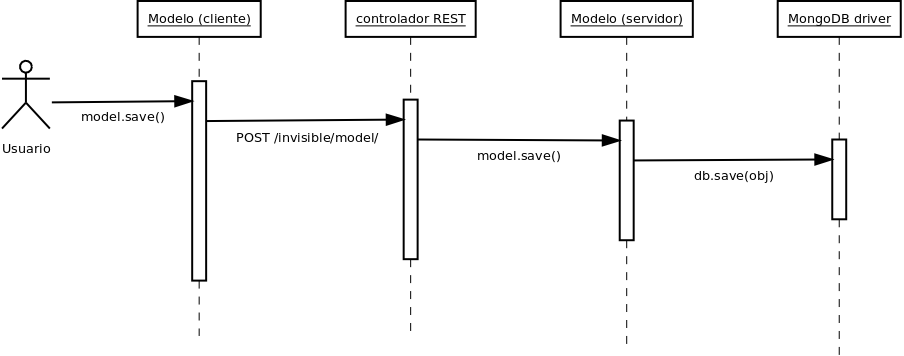
\includegraphics[width=1\columnwidth]{tpprof1.png}
\caption{Secuencia de llamados para un método en el cliente}

\end{center}
\end{figure}

\subsection{Tercera iteración}
\subsubsection{Repositorio público}
El código fuente se maneja con el sistema de control de versiones distribuido Git\cite{git}, a través del sitio Github\cite{github}. Este sitio favorece a sus usuarios en la tarea del desarrollo colaborativo, proveyendo herramientas online para realizar forks y pull requests, reportar bugs, proponer mejoras, etc., siendo el medio estándar para desarrollo del movimiento Open Source en la actualidad. A fin de de habilitar la futura difusión del proyecto, se comenzó a escribir su documentación pública en la portada del proyecto en ese sitio\cite{invisible}. Se planea extender esta documentación en las iteraciones subsiguientes.

También se registró el proyecto en npm, el gestor de paquetes de Node.js, facilitando la instalación del framework en cualquier proyecto Node.js que quiera utilizarlo, siguiendo las prácticas habituales de la comunidad.

\subsubsection{Unit Testing e Integración continua}
Es vital que cualquier proyecto posea una cantidad importante de tests, que garanticen la confiabilidad y robustez del framework. En particular, al tratarse de un proyecto Open Source, donde son varias las personas que pueden agregar código al proyecto (y, por lo tanto, introducir errores), es de suma importancia que los tests sean fáciles de ejecutar, de programar, y que además esté garantizado de que se corran antes de que nuevo código sea aceptado en el proyecto.

Para cumplir estos objetivos, se utilizaron varias herramientas:
\begin{itemize}
\item  Mocha\cite{mocha}: Se trata de un framework de testing flexible y poderoso. Permite escribir tests utilizando la metodología BDD (Desarrollo basado en comportamiento), que es una extensión de TDD (Desarrollo basado en Tests), pero en el cual se incentiva que los test sean descritos de una forma particular. El framework va a ejecutar todos los tests y mostrar un informe en pantalla de con las ejecuciones que fueron exitosas, y también las que fallaron (en este último caso, nos va a proporcionar más información, como por ejemplo el nombre de la excepción que fue lanzada, o la aserción incorrecta).
\item  Grunt\cite{grunt}: Se trata de una herramienta de uso general para ejecución de tareas en JavaScript. Su objetivo es automatizar en mayor medida el ciclo de desarrollo de un proyecto. Nosotros lo usamos, entre otras cosas, para ejecutar los tests de mocha automáticamente en el momento que se hace un cambio local.
\item  Travis\cite{travis}: Es trata de un servicio de Integración Continua (CI) especialmente útil ya que tiene integración con Github. Cada vez que alguien proponga un cambio de código en nuestro servidor (un pull request), el servicio va a levantar un servidor con el código propuesto, correr todos los tests, e informar si el cambio propuesto es seguro (es decir, se pasó todos los tests exitosamente).  

\end{itemize}
\subsubsection{Diseño de la aplicación de ejemplo}
Habiéndose sentado las bases del framework, se hace necesario para extenderlo y corregirlo, basarse en su utilización en un sistema real. Para ello, en esta iteración comenzamos a planificar una aplicación de ejemplo que se adecúe a tal fin.

En primera instancia se consideró implementar una aplicación de gestión de casos de prueba, similar a la  trabajada en el marco laboral, según se documentó en la etapa de prototipos. Sin embargo se descartó esta idea, por representar un tamaño de trabajo demasiado amplio que cubrir, con un aprovechamiento limitado de las características del framework.

Se optó, en cambio, por implementar una aplicación de chat, con manejo de usuarios, contactos y “salones”. La ventaja de este tipo de sistema es que su tamaño es reducido, sin demasiado diseño gráfico, y con mucha dinamicidad. El hecho de que se manejen usuarios agrega un componente de formularios y validaciones que interesa estudiar en el proyecto.

La decisión de implementar un chat, hizo que el soporte de sincronización en tiempo real, que hasta ahora se consideraba funcionalidad secundaria del framework, pase a ser necesaria.

\subsection{Cuarta iteración}
\subsubsection{Arquitectura de la aplicación de ejemplo}
La cuarta iteración se centró en implementar el chat de ejemplo definido anteriormente, y actualizar el framework según esta tarea lo requiera. Se puede sintetizar la arquitectura resultante en las siguientes características:
\begin{itemize}
\item  Los casos de uso son: registrar nuevo usuario, ingresar y salir del sistema, listar y agregar contactos, listar y crear salones, enviar mensaje a un contacto, enviar un mensaje a un salón.
\item  Consta de tres modelos manejados por Invisible.js: User, Room y Message.
\item  La interfaz es una Single-Page app, que usa AngularJS para el ruteo, controladores y templates. El modelo al que están atados esos componentes son en general los modelos de Invisible.js
\item  Para implementar la comunicación bidireccional y las acutalizaciones en tiempo real se crean sockets entre el servidor y los clientes, usando socket.io (ver adelante).

\end{itemize}
\subsubsection{Validaciones}
Una de las tareas donde se hace más evidente el problema que pretende resolver Invisible.js es en el manejo de validaciones: resulta deseable para la mejor experiencia de usuario realizarlas en el cliente, pero a la vez es necesario validar todo lo que llega al servidor antes de guardarlo a la base de datos. En general esto implica duplicar la lógica de validación en ambos lados.

Nos interesa entonces proveer alguna manera de definir validaciones en el modelo, y que estas sean aplicables en ambos contextos. Para eso se integró al modelo extendido de Invisible.js la biblioteca revalidator\cite{revalidator}, que provee una convención sencilla para definir validaciones sobre un objeto JavaScript y un método para ejecutarlas.

Para aplicar validaciones, el usuario del framework debe definir el atributo “validations” que sigue el esquema requerido por revalidator. Luego se extiende el modelo con el método validate, que será llamado antes de salvar el modelo, arrojando un error si el estado no es válido. Por ejemplo:

\begin{lstlisting}
class Person
    constructor: (@name)->
    validations: 
        properties:
            name:
                type: "string"

Invisible.createModel("Person", Person)

person = new Invisible.Person("John")
person.validate() #returns {valid: true, errors: []}

person.name = 5
person.validate() 
#returns {valid: false, errors: [{attribute: 'type', property: #'name', expected: 'string', actual: 'number', message: 'must be of string type'}]}}
person.save() #throws error
\end{lstlisting}

Uno de los mayores avances de la actualidad en lo que a aplicaciones web se refiere el soporte a comunicación en tiempo real. La biblioteca por excelencia que implementa tiempo real en Node.js se llama socket.io. 

En el caso de que uno quiera agregarle funcionalidad de tiempo real a su aplicación, Invisible agregar ciertos métodos a sus modelos que brindan dicho soporte. En particular, agrega los siguientes tres métodos:


\begin{itemize}
\item  Model.onNew: Este método se va a ejecutar cuando se guarde en la base de datos una nueva instancia de la clase Model. Devuelve la instancia creada en la función callback.
\item  Model.update: Este método se va a ejecutar cada vez que una instancia sea modificada. Devuelve la instancia modificada en la función callback.
\item  Model.delete: Este método se va a ejecutar cada vez que una instancia sea eliminada. Devuelve la instancia eliminada en la función callback.

\end{itemize}
\subsection{Quinta iteración}
\subsubsection{Despliegue de la aplicación de ejemplo}


Un paso a tener en cuenta a la hora de desarrollar cualquier aplicación web es poder llevarla a un ambiente de producción sin mayores problemas. No es lo mismo un entorno local de desarrollo que uno remoto, y puede haber algunas dificultades a sortear. Necesitamos que nuestro framework sea lo suficientemente flexible como para poder adaptarse a las particularidades de cada entorno. En el último tiempo se están popularizando soluciones de Cloud Computing que permiten aumentar los recursos de hardware asignados a la aplicación con solo apretar un botón (y pagando más dinero, obviamente). Una de las soluciones más conocidas y usadas es Heroku\cite{heroku}, que es la plataforma que usamos para desplegar nuestra aplicación de ejemplo. 

Dentro de las particularidades de esta plataforma, hubo que tener en cuenta que usa un servidor externo como base de datos, de modo que es necesario que el que ese parámetro sea configurable en el framework. Nosotros usamos el servicio llamado MongoLab\cite{mongolab}, el cual nos provee la url de la base de datos mediante la variable de entorno MONGOLAB\_URI.

Otra de las cuestiones a tener en cuenta es que no todas las plataformas tienen soporte a Websockets. Dado que socket.io implementa el soporte a real time de distintas maneras, esto no es un problema, pero es necesario exponer al usuario las configuraciones para que pueda hacer los cambios pertinentes.

En el caso de Heroku, empezó a soportar WebSockets de forma experimental, y se puede activar corriendo el siguiente comando:

\begin{verbatim}
heroku labs:enable websockets
\end{verbatim}

La aplicación esta deplegada bajo la siguiente dirección: \url{http://invisible-chat.herokuapp.com/}

\section{Desarrollo de una aplicación con Invisible.js}


Habiendo completado el desarrollo de la funcionalidad propuesta para el framework y una aplicación de ejemplo que lo utiliza, nos interesa evaluar los resultados obtenidos. En particular, cómo resulta la experiencia de desarrollar una aplicación usando Invisible.js. Para ello describiremos paso a paso el proceso para una versión reducida del Chat con el que se trabajó anteriormente.

Lo primero consiste en crear un proyecto node.js, para lo cual hay que crear un archivo llamado package.json el cual contiene la metainformación del proyecto y las dependencias necesarias. El nuestro se verá así:

\begin{lstlisting}
{
  "name": "minimalChat",
  "version": "0.0.1",
  "dependencies": {
    "invisible": "*",
    "coffee-script": "~1.6.3",
    "express": "~3.3.4"
  },
  "engines": {
    "node": ">=0.8.0"
  }
}
\end{lstlisting}

Nótese que todo proyecto necesita tener “invisible” y “express” como dependencias, para que el mismo pueda funcionar.

Ahora podemos crear el servidor express, e integrar invisible. Para ello creamos el archivo server.coffee, el cual contiene la siguiente información:

\begin{lstlisting}
express = require("express")
http = require("http")
path = require("path")
invisible = require("invisible")
app = express()

app.set("port", 3000)
app.use(express.bodyParser())
app.use(app.router)
app.use(express.static(path.join(__dirname, "public")))

invisible.createServer app, path.join(__dirname, "models"), {} , () ->
  console.log "Express server listening on port " + app.get("port")
\end{lstlisting}

Vemos que podemos crear nuestra aplicación llamando a la función express, y luego realizamos algunas configuraciones, como setear el puerto al cual el servidor escucha, definir que public va a ser la carpeta estática, entre otros.

Lo más importante es la última línea: 

\begin{lstlisting}
invisible.createServer app, path.join(__dirname, "models"), {} , () ->
  console.log "Express server listening on port " + app.get("port")
\end{lstlisting}

Acá estamos integrando invisible, especificando a su vez la ruta que va a contener nuestros modelos de dominio, en este caso, models. Esta función va a crear un servidor http convencional de node, pero va a agregar todas las configuraciones necesarias para hacer funcionar a Invisible.

Luego se definen los modelos de dominio de la aplicación y se los registra con Invisible.js. Creamos un archivo message.coffee en la carpeta models.

\begin{lstlisting}
Invisible = require("invisible")

class Message
    constructor: (@from, @body) ->
      @date = new Date()

module.exports = Invisible.createModel("Message", Message)
\end{lstlisting}

Con esto basta para resolver la persistencia, autogenerar los controladores REST, publicar en tiempo real los eventos en los modelos. Todas estas tareas se realizarán de manera totalmente transparente para el programador. 

Con los pasos anteriores queda sentada casi en su totalidad la arquitectura de la aplicación. A continuación podemos definir la funcionalidad que tendrá y construir la interfaz que la implemente sirviéndose de las facilidades de Invisible.js.

La aplicación va a consistir en un único salón en el cual interactúan todos los usuarios, a los cuales se les asigna un nombre al azar. Nuestro código de cliente va a consistir entonces de un archivo index.html y otro app.coffee, ambos bajo el directorio public.

\begin{lstlisting}[language=html]
<!doctype html>
  <head>
    <meta charset="utf-8">
    <link href="//netdna.bootstrapcdn.com/bootstrap/3.0.2/css/bootstrap.min.css" rel="stylesheet">
  </head>
  <body ng-app="minimalChat">
    <div class="container" ng-controller="MainCtrl">
      <div class="col-md-8" style="margin-top: 30px;">
        <div class="well well-lg" id="message-list"> 
          <div ng-repeat="message in messages">
            <div class="message-body">
              <small><b ng-bind="message.from"></b></small><small class="pull-right text-muted" ng-bind="message.date|date:'short'"></small><br/>
            </div>
            <div>
              <small ng-bind="message.body"></small>
            </div>
          </div>
        </div>
        <form ng-submit="enterMessage()" class="chat" novalidate>
          <div class="form-group">
            <input type="text" class="form-control chat-input" ng-model="message" required placeholder="Enter message" autofocus>
          </div>    
        </form>
      </div>
    </div>

    <script src="http://code.jquery.com/jquery-1.10.1.min.js"></script>
    <script src="//netdna.bootstrapcdn.com/bootstrap/3.0.2/js/bootstrap.min.js"></script>
    <script src="https://ajax.googleapis.com/ajax/libs/angularjs/1.0.1/angular.min.js"></script>
    <script src="invisible.js"></script>
    <script src="app.js"></script>
  </body>
</html>
\end{lstlisting}

Este es el archivo principal, el cual contiene las referencias a las distintas bibliotecas usadas. Es particularmente interesante la linea general la integración con Invisible:

\begin{lstlisting}[language=html]
<script src="invisible.js"></script>
\end{lstlisting}

Solo con eso, todos nuestros modelos van a podes ser utilizados desde el cliente.

Nuestro código Angular se va a limitar a:

\begin{lstlisting}
angular.module('minimalChat', [])

angular.module('minimalChat')
  .controller 'MainCtrl', ($scope) ->

    $scope.user = "user-" + Math.floor(Math.random()*1000)

    $scope.messages = []
    $scope.message = ''

    $scope.enterMessage = () ->
        message = new Invisible.Message($scope.user, $scope.message)
        message.save (err, res) -> return
        $scope.message = ''
        $scope.messages.push(message)

    Invisible.Message.onNew (message)->
        $scope.$apply () ->
            if message.from != $scope.user
                $scope.messages.push(message)
\end{lstlisting}

\section{Conclusiones}
El presente trabajo resultó fructífero, en primer lugar por habernos dado la posibilidad de estudiar y aplicar tecnologías incipientes que marcan el rumbo del desarrollo web, y también por haber podido llevar adelante el desarrollo integral de un proyecto de software, aplicando los conocimientos adquiridos en el campo académico y profesional, desde una etapa intensa de investigación y evaluación de alternativas hasta un producto final. Vale remarcar a su vez que este producto superó las expectativas iniciales, teniendo valor en sí mismo. Nos interesa, en fin, realizar a modo de conclusión un balance del trabajo realizado y de las posibilidades de extenderlo en adelante.

En primer término hay que destacar que se trabajó sobre un set de tecnologías desarrolladas comunitariamente con un alto dinamismo. Invisible.js propone una forma novedosa de desarrollo de aplicaciones web, pero en cierta medida lo hace combinando distintas herramientas surgidas recientemente y en constante evolución. La contracara de este amplio espectro de recursos disponibles es entrar en un terreno de escasa madurez, en muchos casos teniendo que resolver problemas de proyectos ajenos, que cambian continuamente y no fueron suficientemente probados. Con todo, Invisible.js es producto de esta modalidad de trabajo, y alcanzará su potencial en la medida en que sea difundido y se construya una comunidad que lo sostenga.

A continuación es necesario evaluar Invisible.js, primero de acuerdo a los objetivos trazados para este trabajo, luego como producto de software en sí mismo. Repasemos entonces los objetivos iniciales del proyecto:
\begin{itemize}
\item  Definir una sola vez modelos, validaciones, métodos y consultas a la base de datos, y poder usarlos indistintamente en cliente y servidor. En este aspecto se obtuvieron resultados muy satisfactorios: no sólo se eliminó por completo la duplicación en el código de modelos y validaciones, sino que se provee mucha de esta funcionalidad automáticamente: interacciones con la base de datos que se adaptan al ambiente en que se realizan, un esquema para definir validaciones que se ejecutan antes de guardar datos, tanto en cliente como en servidor, la posibilidad de emplear librerías residentes en el servidor también en el cliente, etc.
\item  Automatizar la actualización de la vista de acuerdo al estado de los datos, sean estos modificados en la vista por cualquier usuario o en el backend. Si bien en algún momento del desarrollo se consideró este objetivo como secundario, con la ayuda de las bibliotecas disponibles se lo implementó a través de una interfaz sencilla, resultando trivial escribir código que reacciona a eventos relativos a la modificación de los modelos.
\item  Definir los templates de las páginas una sola vez, pudiendo precargarlas en el servidor al entrar en una url específica, o actualizarlas arbitrariamente desde el cliente. Este es el único de los objetivos iniciales que quedó obsoleto, en el sentido de que la investigación nos inclinó a no incluir un sistema de templates en la plataforma. Esto se debe a que consideramos más realista que esta se pueda integrar satisfactoriamente con herramientas ya disponibles, como Angular.js. 

\end{itemize}


La arquitectura de Invisible.js prioriza la construcción de APIs REST en el servidor, que son consumidas en el cliente por Single-page apps. Esto implica, en referencia al punto 3 anterior, que deja de ser necesario manejar templates en el servidor. Esto introduce una de las conclusiones más interesantes del trabajo, a saber, la estructura de las aplicaciones que suponíamos resultaría de lograr nuestro objetivo de reducir la diferencia entre cliente y servidor. En efecto, hallamos que al generarse automáticamente los controladores en el servidor, la necesidad de escribir código allí es mínima, concentrándose el desarrollo el cliente. Restaría evaluar esta situación en aplicaciones más complejas, en las que podría ser necesario introducir procesamiento “de fondo” en el servidor, o nuevos controladores para complementar los generados automáticamente.

Como se dijo, para construir un entorno completo de desarrollo usando Invisible.js, se lo debe complementar con algún framework MVC en el cliente, que no imponga mayores restricciones sobre los modelos que utiliza. Por esto, y porque lo consideramos el mejor disponible, en general elegimos Angular.js para esta tarea. Si bien los resultados fueron satisfactorios, existe la posibilidad de realizar esta integración más elegantemente, para aprovechar mejor las características de ambas herramientas. Por ejemplo, para unificar los criterios para implementar validaciones, y para que los modelos de Invisible.js actúen transparentemente sobre el motor de Angular.js.

En cuanto a la utilidad de Invisible.js más allá de la propuesta inicial, como se desprende del tutorial anterior, hay varios puntos que lo hacen una herramienta interesante. Como se indicó, no solo se evita la duplicación de código, sino que un buen porcentaje del desarrollo clásico deja de ser necesario gracias a la funcionalidad autogenerada, al punto que casi no existe código en el servidor. El ciclo de desarrollo consiste más bien en definir los modelos con los que se va a trabajar y utilizarlos en el cliente, según lo requiera la aplicación y el framework que se utilice en ese ambiente. En particular, la sencillez con la que se trabaja con actualizaciones en tiempo real hace que aplicaciones antes engorrosas se vuelvan triviales de implementar con Invisible.js.

Es necesario aún evaluar cuán escalable es la arquitectura propuesta por Invisible.js, así como su implementación actual. Esto se refiere tanto a cómo soporta exigencias de recursos ( usuarios concurrentes, grandes volúmenes de datos) como a la manera en que se adapta al crecimiento de los proyectos que la aplican. En este sentido, sería también interesante estudiar maneras de realizar módulos reusables que usen la plataforma.

Otro aspecto que requiere trabajo futuro, y el que impide actualmente considerar a Invisible.js como una herramienta viable de ser utilizada más allá del ambiente académico o las pruebas de concepto, es el de las medidas de seguridad. En la actual implementación, no hay manera de restringir el acceso a los datos a usuarios autorizados: no hay autenticación ni protección de los datos, bastando abrir una consola en el browser para acceder y hasta destruir todos los datos. De igual manera el acceso a los eventos relacionados a los modelos no está restringido.

\newpage

\section*{Glosario}

\begin{itemize}
\item  CGI: Common Gateway Interface. Método usado por los web servers para delegar la generación del contenido de las páginas a un archivo ejecutable.
\item  DOM: Document Object Model. Modelo que proporciona un conjunto estándar de objetos para representar documentos XML y HTML. Se utiliza como interfaz de programación para acceder y modificar dinámicamente el contenido de los documentos con lenguajes como JavaScript.
\item  MV*: Model View *. Sigla genérica usada para referir conjuntamente al patrón Model-View-Controller y sus derivados, Model-View-Presenter, Model-View-ViewModel, etc.
\item  MVC: Model-View-Controller. Patrón de desarrollo de software que consiste en separar la información (Modelo) de su representación (Vista).
\item  MVVM: Model-View-ViewModel. Derivativo del patrón MVC, que facilita el desarrollo de interfaces gráficas responsivas a eventos.

\end{itemize}

\newpage

\begin{thebibliography}{150}

\bibitem{jsmvcvs}
  \emph{JavaScript MVC: Client vs Server}.
  \url{https://docs.google.com/presentation/d/1K4RY_1dOi2o_0RBPTr05WL0Vr9E28rRJsnbUP23D6hc/edit#slide=id.gf37f796\_147\_0}

\bibitem{rich}
  \emph{Rich Internet Application}.
  \url{http://en.wikipedia.org/wiki/Rich_Internet_application}

\bibitem{richjs}
  Steven Sanderson,
  \emph{Rich Javascript Applications: The Seven Frameworks}.
  \url{http://blog.stevensanderson.com/2012/08/01/rich-javascript-applications-the-seven-frameworks-throne-of-js-2012/}

\bibitem{backbone}
  \emph{Backbone.js}.
  \url{http://backbonejs.org/}

\bibitem{knockout}
  \emph{Knockout}.
  \url{http://knockoutjs.com/}

\bibitem{mvw}
  Addy Osmani,
  \emph{Journey Through The JavaScript MVC Jungle}.
  \url{http://coding.smashingmagazine.com/2012/07/27/journey-through-the-javascript-mvc-jungle/}

\bibitem{wdsucks}
  Harry Brundage,
  \emph{Today, web development sucks}.
  \url{http://harry.me/blog/2011/01/27/today-web-development-sucks/}

\bibitem{node}
  \emph{Node.js}.
  \url{http://nodejs.org/}

\bibitem{coffee}
  \emph{CoffeeScript}.
  \url{http://coffeescript.org/}

\bibitem{websockets}
  Malte Ubl and Eiji Kitamura,
  \emph{Introducing WebSockets: Bringing Sockets to the Web}.
  \url{http://www.html5rocks.com/en/tutorials/websockets/basics/}

\bibitem{goodparts}
  Douglas Crockford,
  \emph{JavaScript: The Good Parts}.

\bibitem{grunt}
  \emph{Grunt, the JavaScript task runner}.
  \url{http://gruntjs.com/}

\bibitem{sourcemaps}
  Ryan Seddon,
  \emph{Introduction to JavaScript Source Maps}.
  \url{http://www.html5rocks.com/en/tutorials/developertools/sourcemaps/}

\bibitem{wsvssse}
  Dmitry Sheiko,
  \emph{WebSockets vs Server-Sent Events vs Long-polling}.
  \url{http://dsheiko.com/weblog/websockets-vs-sse-vs-long-polling}

\bibitem{longpolling}
  \emph{Push technology}.
  \url{http://en.wikipedia.org/wiki/Push_technology}

\bibitem{sse}
  Eric Bidelman,
  \emph{Stream Updates with Server-Sent Events}.
  \url{http://www.html5rocks.com/en/tutorials/eventsource/basics/}

\bibitem{congress}
  Luigi Montanez,
  \emph{Case Study: Real-time Updates in Stream Congress}.
  \url{http://www.html5rocks.com/en/tutorials/casestudies/sunlight_streamcongress/}

\bibitem{wsvssse2}
  \emph{WebSockets vs. Server-Sent events/EventSource}.
  \url{http://stackoverflow.com/questions/5195452/websockets-vs-server-sent-events-eventsource}

\bibitem{ssedownside}
  \emph{Downside of using Server-Sent events for bidirectional client-server communication (instead of WebSockets)}.
  \url{http://stackoverflow.com/questions/13278365/downside-of-using-server-sent-events-for-bidirectional-client-server-communicati}

\bibitem{socketio}
  \emph{Socket.IO}.
  \url{http://socket.io/}

\bibitem{rest}
  Leonard Richardson and Sam Ruby
  \emph{RESTful Web Services}.

\bibitem{template}
  \emph{Web template system}.
  \url{http://en.wikipedia.org/wiki/Web_template_system}

\bibitem{logicless1}
  \emph{What's the advantage of Logic-less template (such as mustache)?}.
  \url{http://stackoverflow.com/a/4946409/993769}

\bibitem{logicless2}
  Satish Pottavathini,
  \emph{The Case Against Logic-less Templates}.
  \url{http://www.ebaytechblog.com/2012/10/01/the-case-against-logic-less-templates/}

\bibitem{clientside}
  Pascal Deschenes,
  \emph{On Client Side Templating}.
  \url{http://blog.rassemblr.com/2011/04/on-client-side-templating/}

\bibitem{dust}
  Veena Basavaraj,
  \emph{Leaving JSPs in the dust: moving LinkedIn to dust.js client-side templates}.
  \url{http://engineering.linkedin.com/frontend/leaving-jsps-dust-moving-linkedin-dustjs-client-side-templates}

\bibitem{template2}
  \emph{Template Engines}.
  \url{http://codingarchitect.wordpress.com/2012/10/22/template-engines/}

\bibitem{nodenormals}
  Saadiq Rodgers-King,
  \emph{Node for normals}.
  \url{http://blog.nodejitsu.com/node-for-normals}

\bibitem{nodeunderstand}
  Felix Geisendörfer,
  \emph{Understanding node.js}.
  \url{http://debuggable.com/posts/understanding-node-js:4bd98440-45e4-4a9a-8ef7-0f7ecbdd56cb}

\bibitem{nodeboss}
  Felix Geisendörfer,
  \emph{Felix's Node.js Convincing the boss guide}.
  \url{http://nodeguide.com/convincing_the_boss.html}

\bibitem{nodephilosophy}
  Charlie Robbins,
  \emph{The Node.js philosophy}.
  \url{http://blog.nodejitsu.com/the-nodejs-philosophy}

\bibitem{npm}
  \emph{Node Packaged Modules}.
  \url{https://npmjs.org/}

\bibitem{githubstars}
  Dan Nanni, 
  \emph{Most popular open-source projects hosted at GitHub}.
  \url{http://xmodulo.com/2013/09/popular-open-source-projects-hosted-github.html}

\bibitem{nodeodd}
  Andrew Munsell, 
  \emph{The (Odd) State of Node.js and its Frameworks}.
  \url{http://www.andrewmunsell.com/blog/the-odd-state-of-nodejs-and-its-frameworks/#.UQFEO2LhrXQ}

\bibitem{nodefws}
  Tyler Renelle, 
  \emph{Node.js frameworks comparison}.
  \url{http://ocdevel.com/blog/nodejs-frameworks-comparison}

\bibitem{express}
  \emph{Express, web application framework for node}.
  \url{http://expressjs.com/}

\bibitem{tower}
  \emph{Tower}.
  \url{http://towerjs.org/}

\bibitem{derby}
  \emph{Derby}.
  \url{http://derbyjs.com/}

\bibitem{meteor}
  \emph{Meteor}.
  \url{http://meteor.com/}

\bibitem{derbymeteor}
  Nate Smith y Brian Noguchi,
  \emph{Our take on Derby vs. Meteor}.
  \url{http://blog.derbyjs.com/2012/04/14/our-take-on-derby-vs-meteor/}

\bibitem{derbyrant1}
  Ben Ellis,
  \emph{Rant: Backbone, Angular, Meteor, Derby}.
  \url{https://gist.github.com/ble/4457840}

\bibitem{derbyrant2}
  Tyler Renelle,
  \emph{Response to the rant}.
  \url{https://gist.github.com/4457396}

\bibitem{flatiron}
  \emph{Flatiron}.
  \url{http://flatironjs.org/}

\bibitem{flatironintro}
  Charlie Robbins,
  \emph{Introducing Flatiron}.
  \url{http://blog.nodejitsu.com/introducing-flatiron}

\bibitem{isomorphic}
  Charlie Robbins,
  \emph{Scaling Isomorphic Javascript Code}.
  \url{http://blog.nodejitsu.com/scaling-isomorphic-javascript-code}

\bibitem{isomorphic}
  Addy Osmani,
  \emph{Developing Backbone.js Applications}.

\bibitem{angular}
  \emph{AngularJS}.
  \url{http://docs.angularjs.org/}

\bibitem{directive}
  \emph{Creating Custom Directives}.
  \url{http://docs.angularjs.org/guide/directive}

\bibitem{knockoutso}
  \emph{Knockout.js tagged questions}.
  \url{http://stackoverflow.com/questions/tagged/knockout.js}

\bibitem{angularso}
  \emph{AngularJS tagged questions}.
  \url{http://stackoverflow.com/questions/tagged/angularjs}

\bibitem{emberso}
  \emph{Ember.js tagged questions}.
  \url{http://stackoverflow.com/questions/tagged/ember.js}

\bibitem{fodder}
  \emph{Fodder}.
  \url{https://github.com/facundoolano/fodder}

\bibitem{flask}
  \emph{Flask, web development, one drop at a time}.
  \url{http://flask.pocoo.org/}

\bibitem{pubsub}
  \emph{Publish–subscribe pattern}.
  \url{http://en.wikipedia.org/wiki/Publish%E2%80%93subscribe_pattern}

\bibitem{redis}
  \emph{Redis}.
  \url{http://redis.io/}

\bibitem{handlebars}
  \emph{handlebars}.
  \url{http://handlebarsjs.com/}

\bibitem{arqrepo}
  \emph{drymodels}.
  \url{https://github.com/facundoolano/drymodels}

\bibitem{arqdoc}
  \emph{TP Arquitectura}.
  \url{https://docs.google.com/document/d/14jvEphmMU-X22szfy1xyjX3of6eEq7ezoB_U6skHt9k/edit?usp=sharing}

\bibitem{spa}
  \emph{Single-page application}.
  \url{http://en.wikipedia.org/wiki/Single-page_application}

\bibitem{mongoose}
  \emph{mongoose, elegant mongodb object modeling for node.js}.
  \url{http://mongoosejs.com/}

\bibitem{acekia}
  \emph{Acekia, the missing test management tool}.
  \url{http://acekia.com/}

\bibitem{mongo}
  \emph{mongoDB}.
  \url{http://www.mongodb.org/}

\bibitem{sandbox}
  \emph{Sandbox (computer security)}.
  \url{http://en.wikipedia.org/wiki/Sandbox_(computer_security)}

\bibitem{browserify}
  \emph{browserify}.
  \url{https://github.com/substack/node-browserify}

\bibitem{require}
  \emph{Require.js, a JavaScript module loader}.
  \url{http://requirejs.org/}

\bibitem{nodemongo}
  \emph{The Node.JS MongoDB Driver Manual}.
  \url{http://mongodb.github.io/node-mongodb-native/}

\bibitem{revalidator}
  \emph{Revalidator}.
  \url{https://github.com/flatiron/revalidator}

\bibitem{git}
  \emph{Git (software)}.
  \url{http://en.wikipedia.org/wiki/Git_(software)}

\bibitem{github}
  \emph{Github}.
  \url{https://github.com/}

\bibitem{invisible}
  \emph{Invisible.js}.
  \url{https://github.com/invisiblejs/invisible}

\bibitem{heroku}
  \emph{Heroku, Cloud computing designed and built for developers}.
  \url{https://www.heroku.com/}

\bibitem{mongolab}
  \emph{mongolab}.
  \url{https://mongolab.com/welcome/}

\bibitem{mocha}
  \emph{mocha}.
  \url{http://visionmedia.github.io/mocha/}

\bibitem{travis}
  \emph{Travis CI, Free Hosted Continuous Integration Platform for the Open Source Community}.
  \url{https://travis-ci.org/}

\end{thebibliography}

\end{document}